\section{Design Model}

%%%%%%%%%%%%%%%%%%%%%%%%%%%%%%%%%%%%%%%
\subsection{Components and Overall Structure}
\label{sec:components}

In this section we show the overal structure of the design. The design is going
to be implemented in Java and Jess. The inference knowledge and domain knowledge
is mostly in the Jess part, while the task knowledge and user interaction is in
the Java part.

The modular structure can be seen in figure~\ref{fig:dm:modules}. The main
applicaton is implemented in Java with a model-view-controller design, see
section~\ref{sec:app}. The model part starts a Jess engine and loads facts and
rules that implement the system model and inferences over it.

In the working memory of the Jess engine are the domain rules, Jess facts
that represent inferential knowledge of car, and the domain parts, Jess facts
with knowledge about the current status of parts of the car.
Domain rules are not modified over a run of the program, while domain parts are modified. 

Information from the Java application goes to Jess by asserting support facts,
these are then interpeted as modifications of domain parts by support rules.
Information from Jess goes to the Java application by Jess queries made by that
application. 

The components in Jess are divided between a engine and a domain part. The
domain parts consists of the domain rules and the domain parts, these are implementations
of templates supplied by the engine. The engines Jess rules do forward and
backward reasoning on these domain rules and domain parts, see section \ref{sec:inferences}.
The domain rules and domain parts can be substituted by rules and parts from a
different domain while keeping the engine. The rules might be understandable by an
expert or user, as our car repair hobbyist does. The complexity of the inferences
made by the engine are not visible in the domain part.

\begin{figure}[htbp]
    \centering
    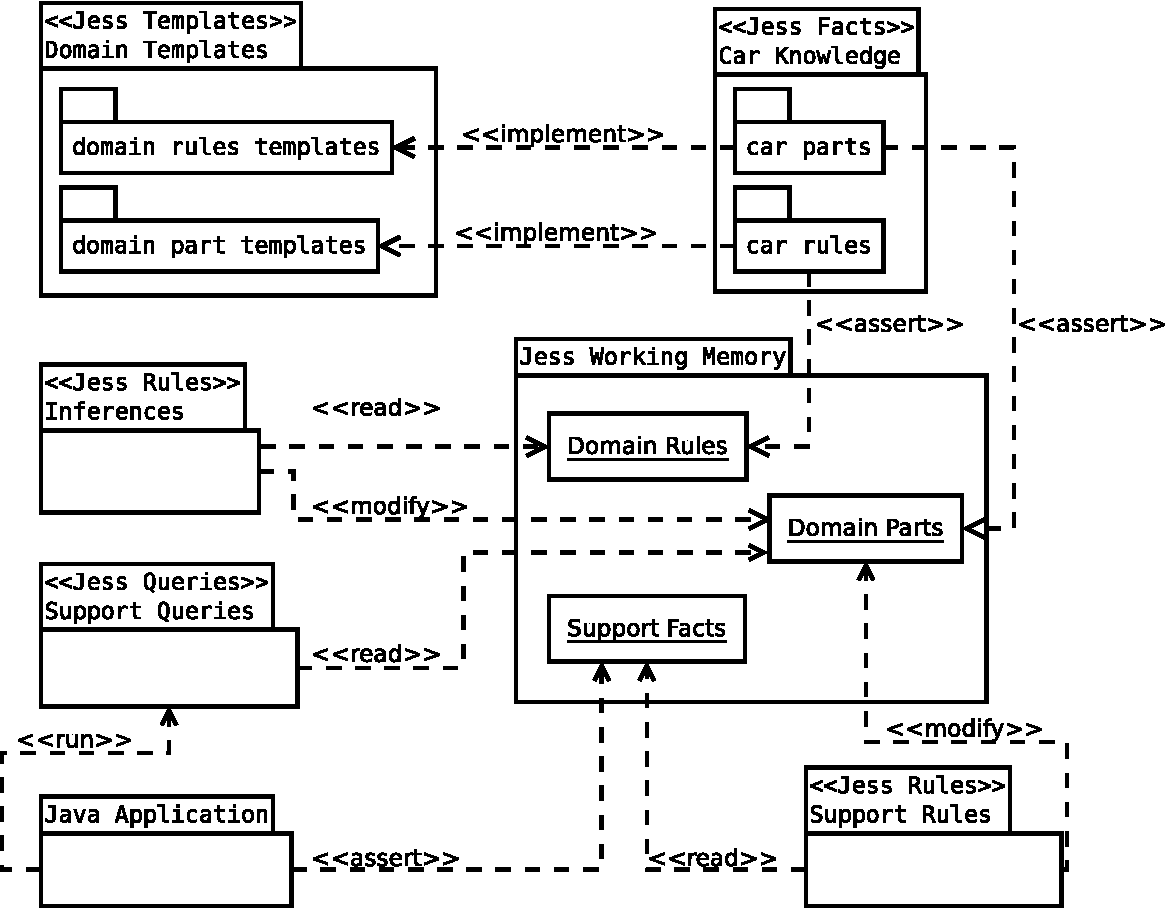
\includegraphics[width=1.00\textwidth]{dm-modules}
    \caption{The modular structure of the design model}
    \label{fig:dm:modules}
\end{figure}

%%%%%%%%%%%%%%%%%%%%%%%%%%%%%%%%%%%%%%%
\subsection{The process flow}
\label{sec:flow}

The overall flow of the application can be seen in the activity diagram in
figure~\ref{fig:dm:activity diagram}. It is based on the communication plan in figure~\ref{fig:communicationPlan}
and the task method in figure~\ref{fig:taskMethod}.

The process start when a complaint is reported to the system. The system then covers
all hypothesis that follow from the complaint. The rest of the process is one
big loop. It has two exits, when a succesfull repair is made, and when there are
no viable hypothesis left. Inside the main loop, first, a hypothesis is selected with
user assistance. Secondly an attempt is made to make an observation, this is a
loop where the user is asked to observe all the possible observables one after
another. If the user want do do an observation the result is used to update all
hypothesis in the verify activity. If the user doesn't want do to any of the
observations or there are no observables for the hypothesis, the user is asked
to repair his or her car. If this repair is succesfull the problem is solved and
the program exits. If the repair isn't succesfull, the hypothesis is considered
impossible by the system.

\begin{figure}[htbp]
    \centering
    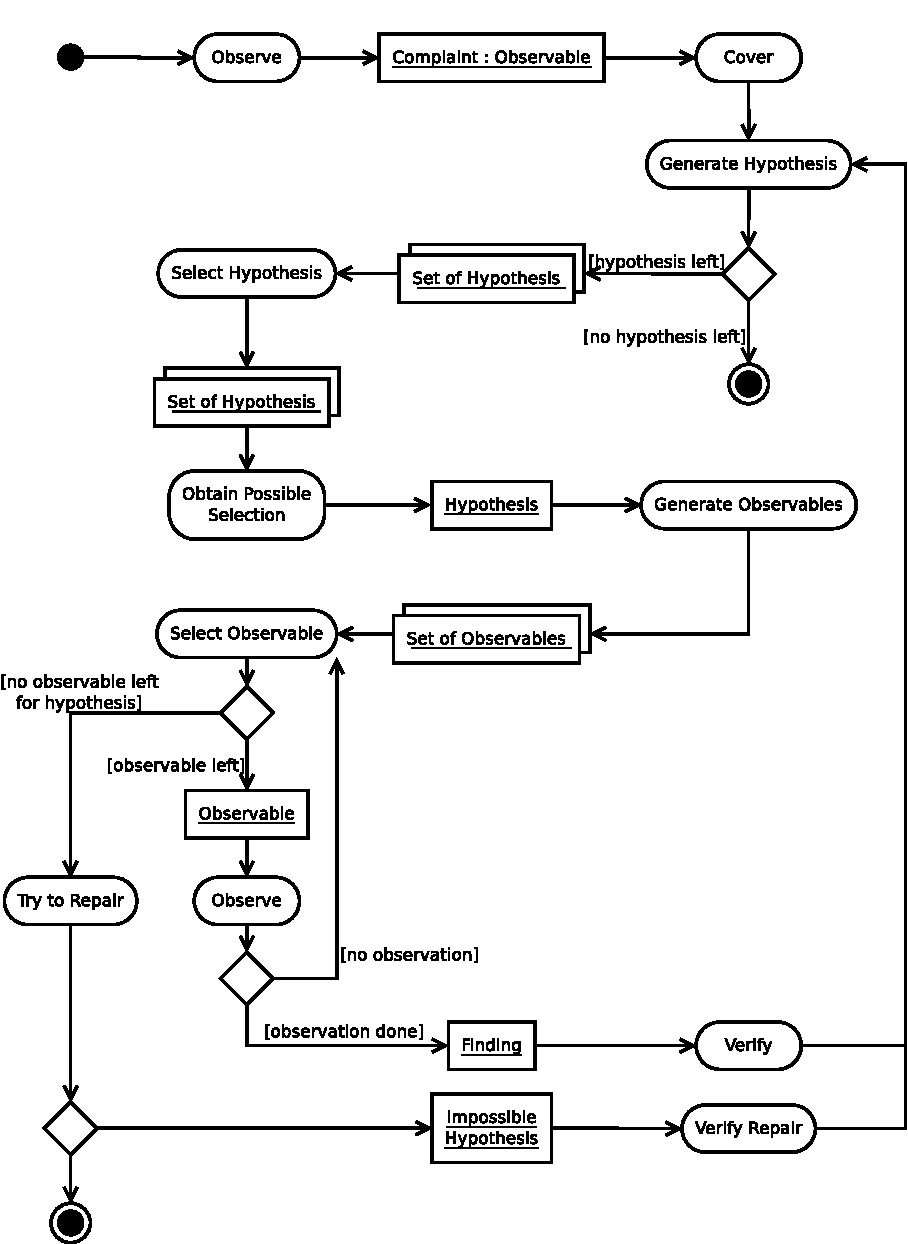
\includegraphics[width=1.00\textwidth]{dm-activity}
    \caption{The overal activity diagram of the application}
    \label{fig:dm:activity diagram}
\end{figure}

%%%%%%%%%%%%%%%%%%%%%%%%%%%%%%%%%%%%%%%
\subsection{The application}
\label{sec:app}

The application is implemented in Java, it's class diagram in figure~\ref{fig:dm:class diagram}.
The model-view-controller pattern is applied. Model keeps all the inference and
domain knowledge of the system. The Java class Model is partly an interface to the part of the model
that is implemented in Jess and partly implements the model
itself, as explained in section~\ref{sec:inferences} and \ref{sec:components}.
Control manages the process flow described in the previous section, and
communicates with Model and View. View implements the user interface and controls the user
interaction if the model is not involved.

\begin{figure}[htbp]
    \centering
    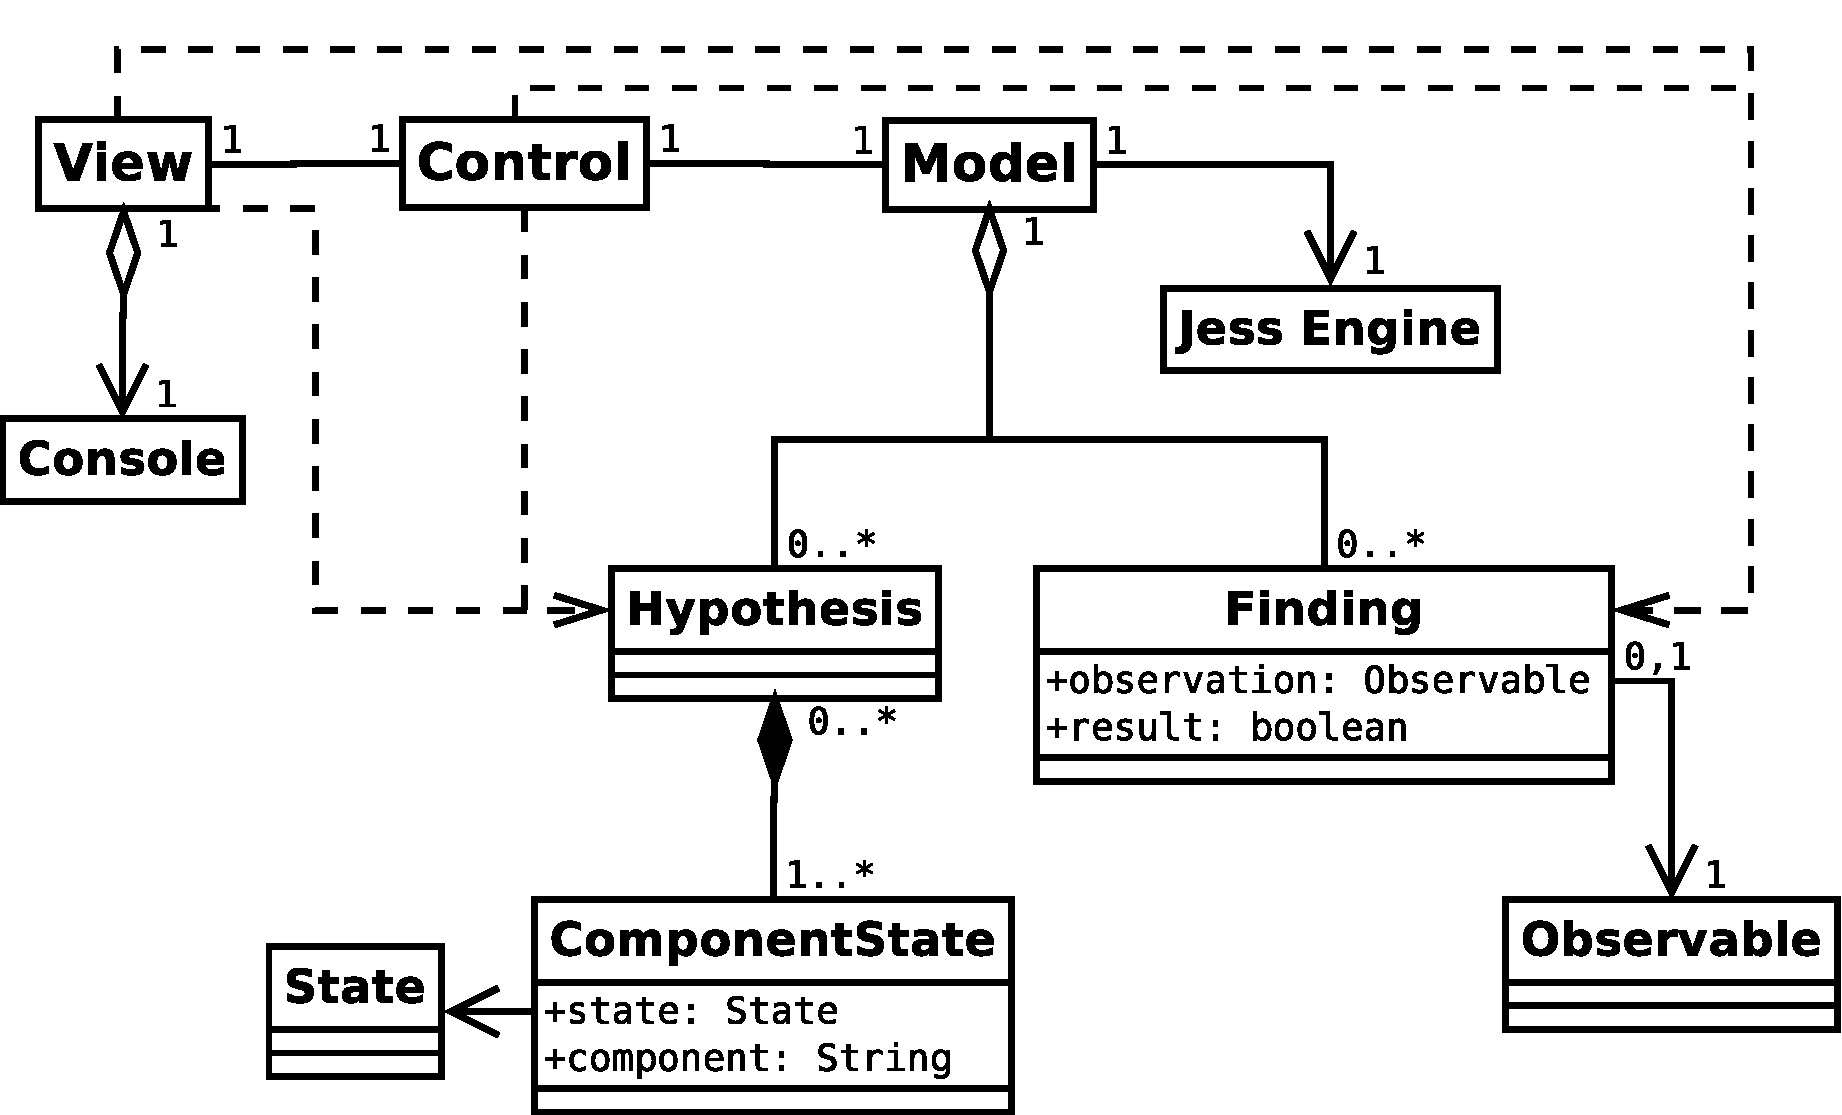
\includegraphics[width=1.00\textwidth]{dm-class}
    \caption{The class diagram of the Java application}
    \label{fig:dm:class diagram}
\end{figure}

The Console class is used for writing and reading from the console. It's mainly
used because java.io.Console is not universily supported. The Jess Engine a Jess
Rete engine from the Jess library. ComponentState is a certain domain part in a
(faulty) state, it wraps a identifier used in the Jess model and a pretty
printable name. An hypothesis consists of one or more parts in a fauly state.
The Hypothesis class  is a list of ComponentStates, it also includes methods operating on
a Hypothesis or a list of Hypothesis. Model delegates a considerable part of its
functionality to Hypothesis. The Observable class wraps an identifier used in the Jess model and a pretty
printable name. The Finding class references an Observable that has been
observed and the result of that observation.

The activity diagram of figure~\ref{fig:dm:activity diagram} is further detailed
in three sequence diagrams showing the interaction between the components Model, View and
Controller.

The first diagram, in figure~\ref{fig:dm:sd cover}, shows how a complaint is
reported and covered, it details the report and cover activities. First Model
is asked for likely complaints, these complaints are shown to the user by View.
The users selects an complaint from this list or enters a new one. The complain
is asserted to model, which automaticly covers it.

The second diagram, in figure~\ref{fig:dm:sd select}, shows how hypothesis are generated
and selected for testing, it details the generate hypothesis, select hypothesis
and obtain possible selection activities. First Model is asked to generate all
possible hypothesis. From these hypothesis one is picked as the default. Then
the user is asked by View wether he wants the system to test the default
hypothesis or wants to select another one, this results in a hypothesis that can
be tested.

The third diagram, in figure~\ref{fig:dm:sd observe}, shows how observations are
negotiated, attempts to repair are done and hypothesis verified by the
results of these two, it details the select observable, try to repair, observe
and verify activities. First a list of all  possible observables for the
hypothesis that is obtained from Model. In the loop the user is asked to observe one of
these observables one after another, until he or she agrees to observe or there
are no more observables left for the hypothesis. If the user agreed to do an
observation this results in a Finding, that is asserted to Model. If there were
no observable the user wants to observe for this hypothesis the user is asked to
repair the car. If this repair is succesfull, the user is congratualed by the
application and can exit. If the repair is unsuccesfull it is assumed the
hypothesis is false from now on, so it's asserted as impossible in Model. After
all this some hypothesis might require removal, because they are not possible
anymore, therefore the model is asked to verify all hypothesis.

\begin{figure}[htbp]
    \centering
    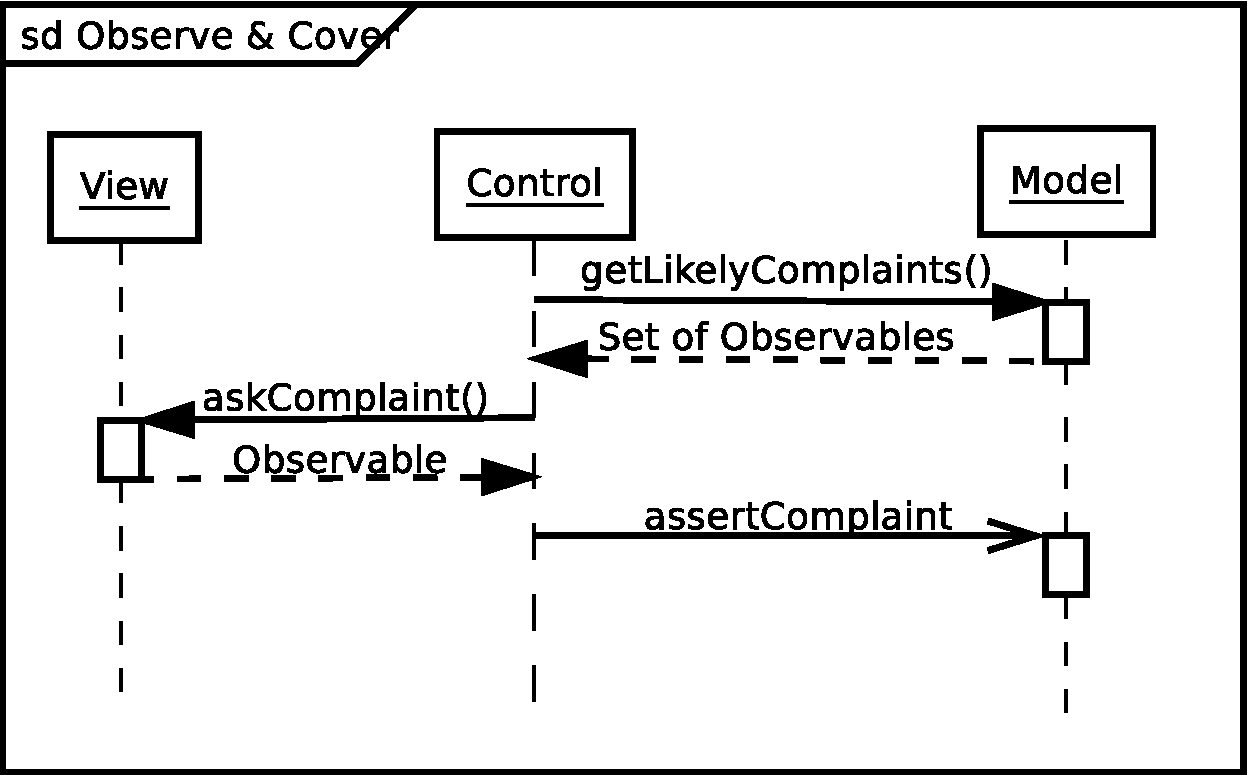
\includegraphics[width=1.00\textwidth]{dm-sd-cover}
    \caption{The sequence diagram detailing report and cover}
    \label{fig:dm:sd cover}
\end{figure}

\begin{figure}[htbp]
    \centering
    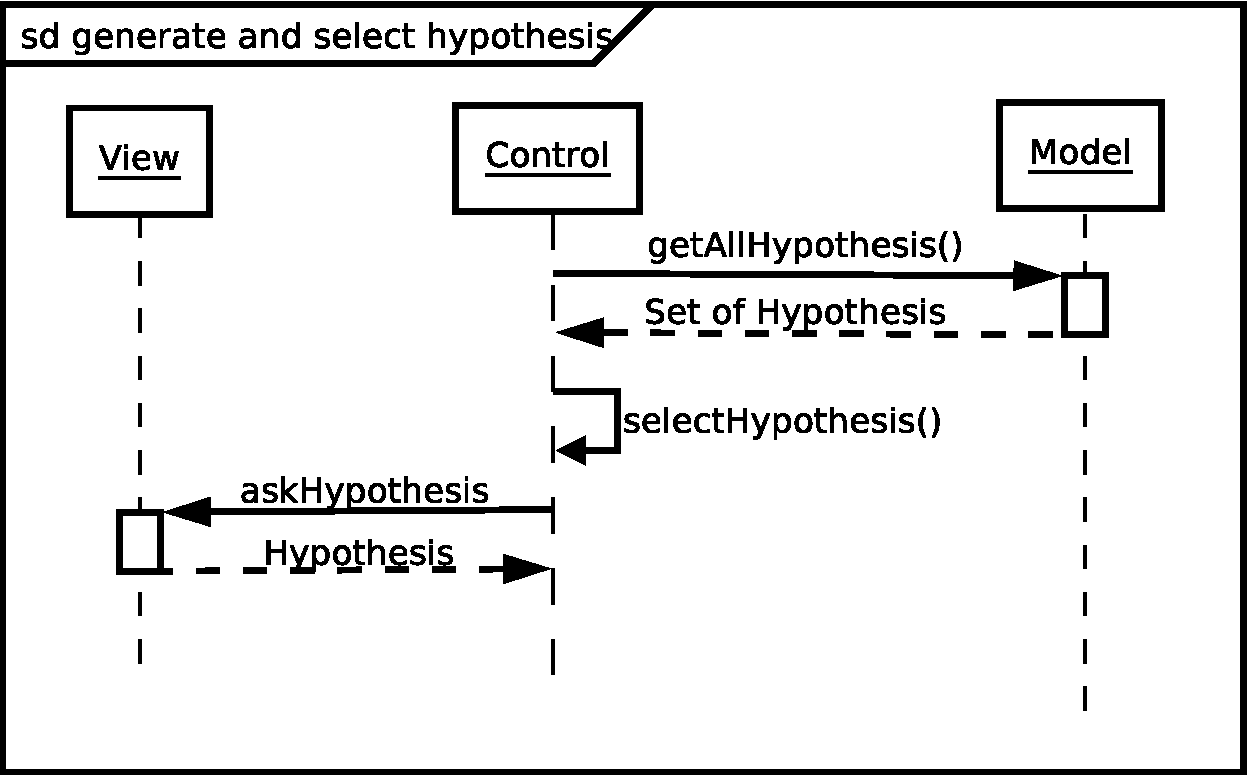
\includegraphics[width=1.00\textwidth]{dm-sd-select}
    \caption{The sequence diagram detailing generating and selecting hypothesis}
    \label{fig:dm:sd select}
\end{figure}

\begin{figure}[htbp]
    \centering
    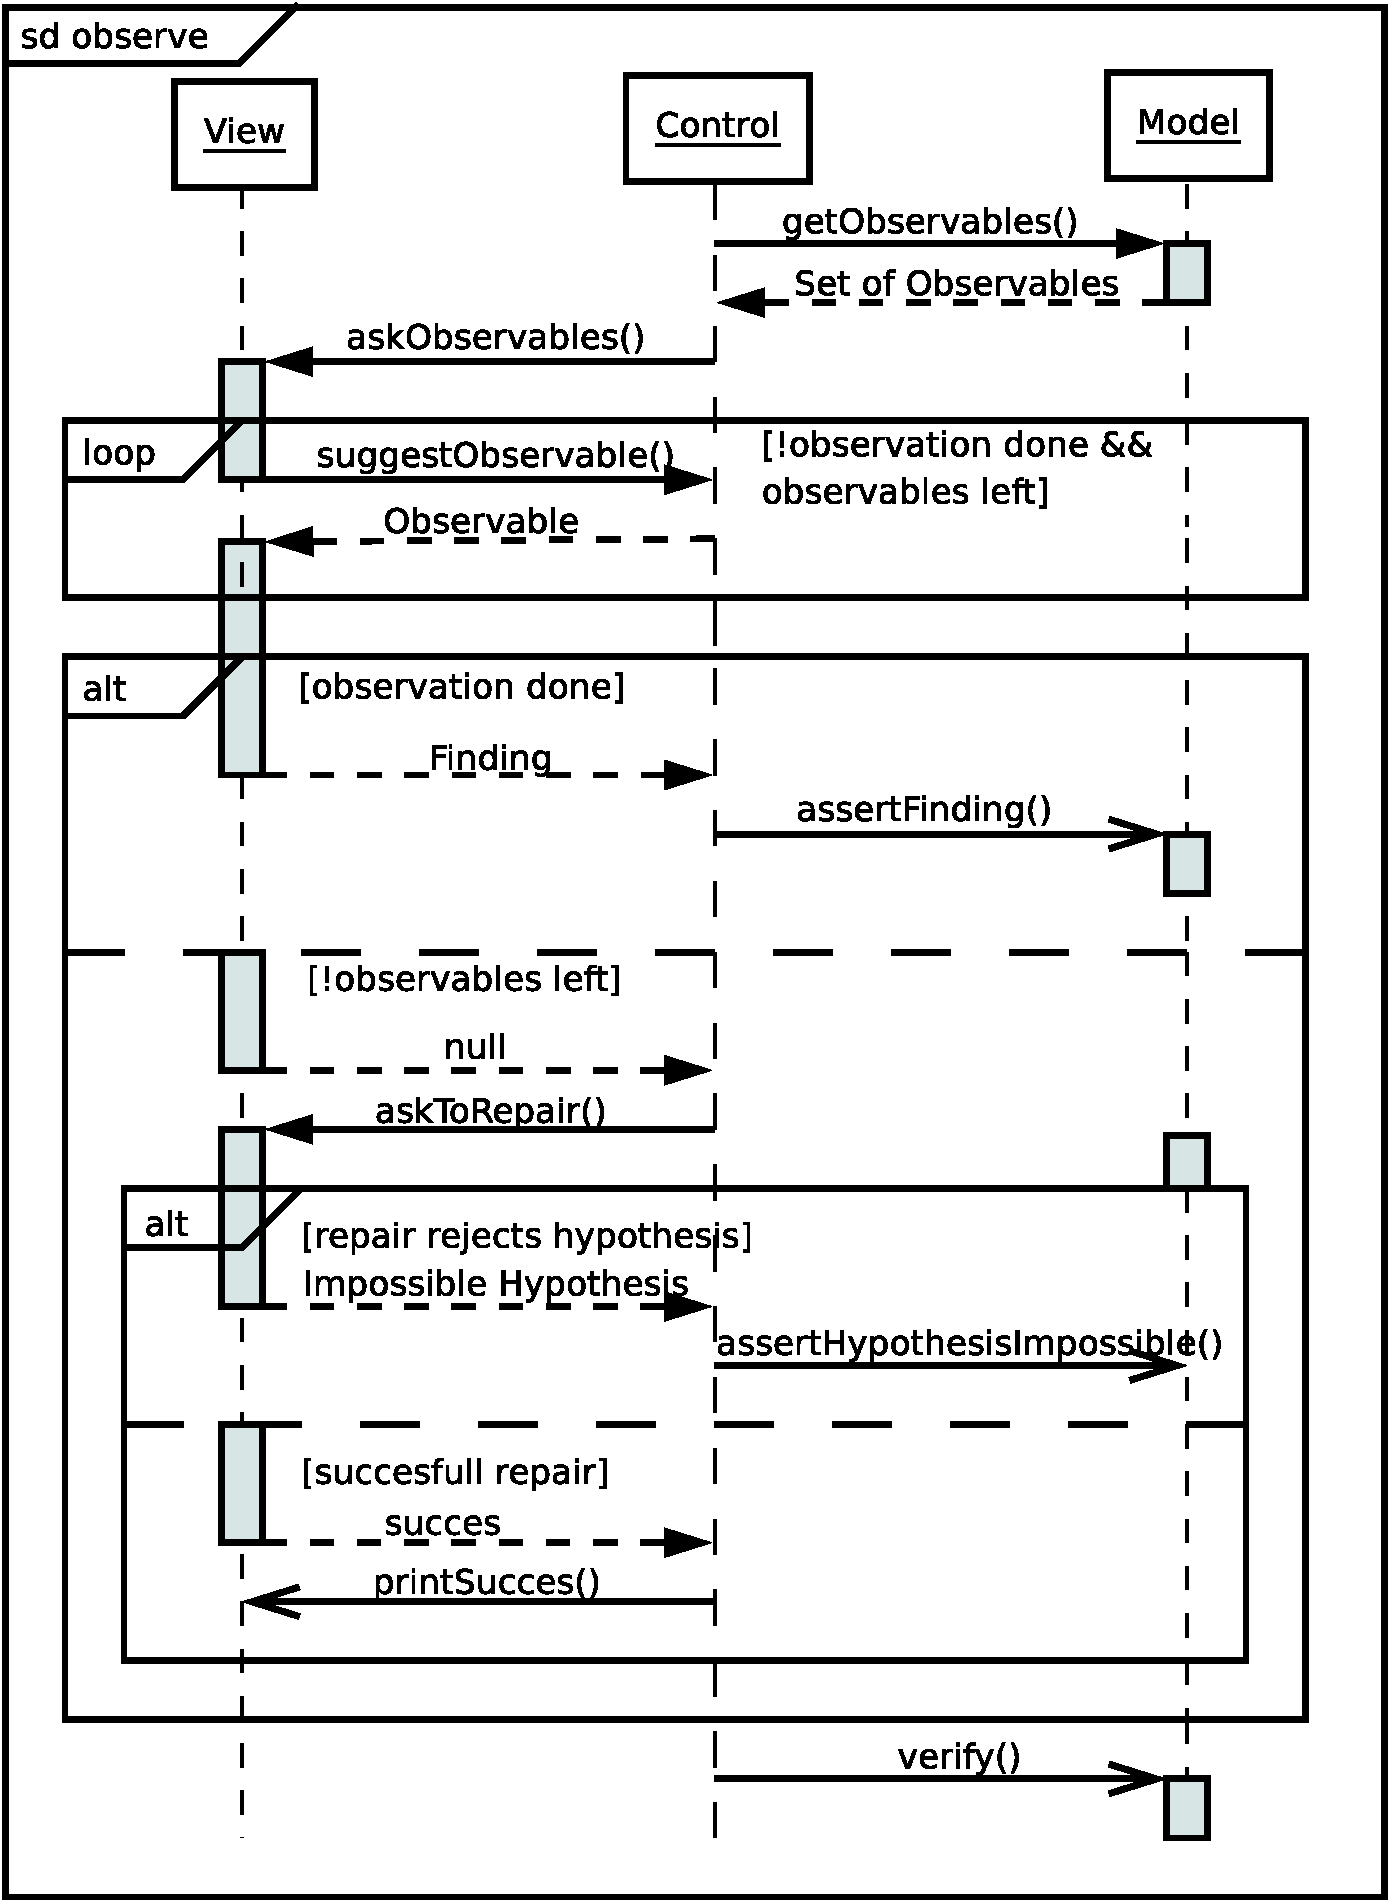
\includegraphics[width=1.00\textwidth]{dm-sd-observe}
    \caption{The sequence diagram detailing observations, try to repair and verify}
    \label{fig:dm:sd observe}
\end{figure}
